\chapter{ROS packages}
ROS komt met een aantal handige packages (libraries) die het werken met en het programmeren van robots makkelijker maken. In dit hoofdstuk kijken we naar de transform library bekent als tf2\footnote{\url{https://wiki.ros.org/tf2} ; Pas op: de meeste voorbeelden op deze link zijn met ROS 1.}

\section{Tf2}
Tf2  (\underline{t}rans\underline{f}orm library 2) is een ROS package (library) die helpt bij het omrekenen van verschillende coördinatensystemen naar elkaar. Dit is erg handig als we werken met hardwarecomponenten die moet samenwerken in de echte wereld. Deze sectie beschrijft wanneer je tf2 nodig hebt en hoe je tf2 gebruikt.

\subsection{Meerdere coördinatensystemen}
Elk hardwarecomponent dat interacteert met de wereld heeft zijn eigen \textit{coordinate frame of reference} of kortweg \textit{coordinate frame}. Hiermee bedoelen we dat elk hardwarecomponent zijn eigen nulpunt (referentiekader) heeft waar vanuit hij redeneert waar andere objecten staan. Zo zal een robotarm die op de HAN in Arnhem waarschijnlijk zeggen dat zijn middelpunt\footnote{Midden- versus middel-: \url{https://www.schrijfwijzer.nl/taalvragen/verwarwoordenboek/verwarwoord/362/middel-midden}} van zijn base de coordinaten (0, 0, 0) heeft. Hiermee bedoelen we dat zijn coordinate frame op het middelpunt van zijn frame zit. Deze locatie van de coordinate frame is logisch voor de robotarm, maar onlogisch voor de rest van de wereld. Zeker als de arm schuin op een tafel is bevestigd op GPS coordinaten (51.98673585896382, 5.951850752998225) en op Rijksdriehoekcoördinaten\footnote{zie voor informatie over Rijksdriehoekcoördinaten: \url{https://nl.wikipedia.org/wiki/Rijksdriehoeksco\%C3\%B6rdinaten}. GPS en Rijksdriehoekcoördinaten hebben ieder ook een andere referentiekader.} (193787, 444411). Het werken met een coordinate frame voor een robotarm maakt veel dingen makkelijker. De robotarm hoeft niet te achterhalen waar in de wereld het is. Alles wat het moet doen kan worden beredeneert vanuit zijn eigen locatie. 

Deze egoïstische kijk van een component op coordinate frames geven wel uitdagingen als er meerdere hardwarecomponenten zijn die moeten samenwerken. Elk hardwarecomponenten heeft namelijk zijn eigen coordinate frame en dus een eigen nulpunt. De coördinaten waar een sensor een object ziet komt dan niet overeen met de coördinaten waar de robotarm heen moet bewegen om het object aan te raken. Dit wordt nog ingewikkelder als we de oriëntatie (Pitch, Yaw en Roll) ook meenemen. Sensors en actuatoren staan vaak in verschillende hoeken. Maar het kan erger. Het is ook mogelijk dat de locatie van een coordinate frame in de echte wereld steeds verandert. Bijvoorbeeld bij een sensor bevestigt op de ``hand'' van een robotarm.

Tf2 helpt ons met het managen van de vele coordinate frames die een robot kan hebben. Het geeft de mogelijkheid om coordinate frames van de verschillende (bewegende) onderdelen naar elkaar of naar een gezamelijke coordinate frame (veelal \textit{world frame} genoemd) om te zetten. In figuur \ref{fig:coordinateframes} zien we een robot met verschillende coordinate frames. De groene, blauwe en rode cilinders  geven de oriëntatie en locaties van de (nulpunten) van de verschillende coordinate frames aan.

\begin{figure}[ht]
\begin{center}
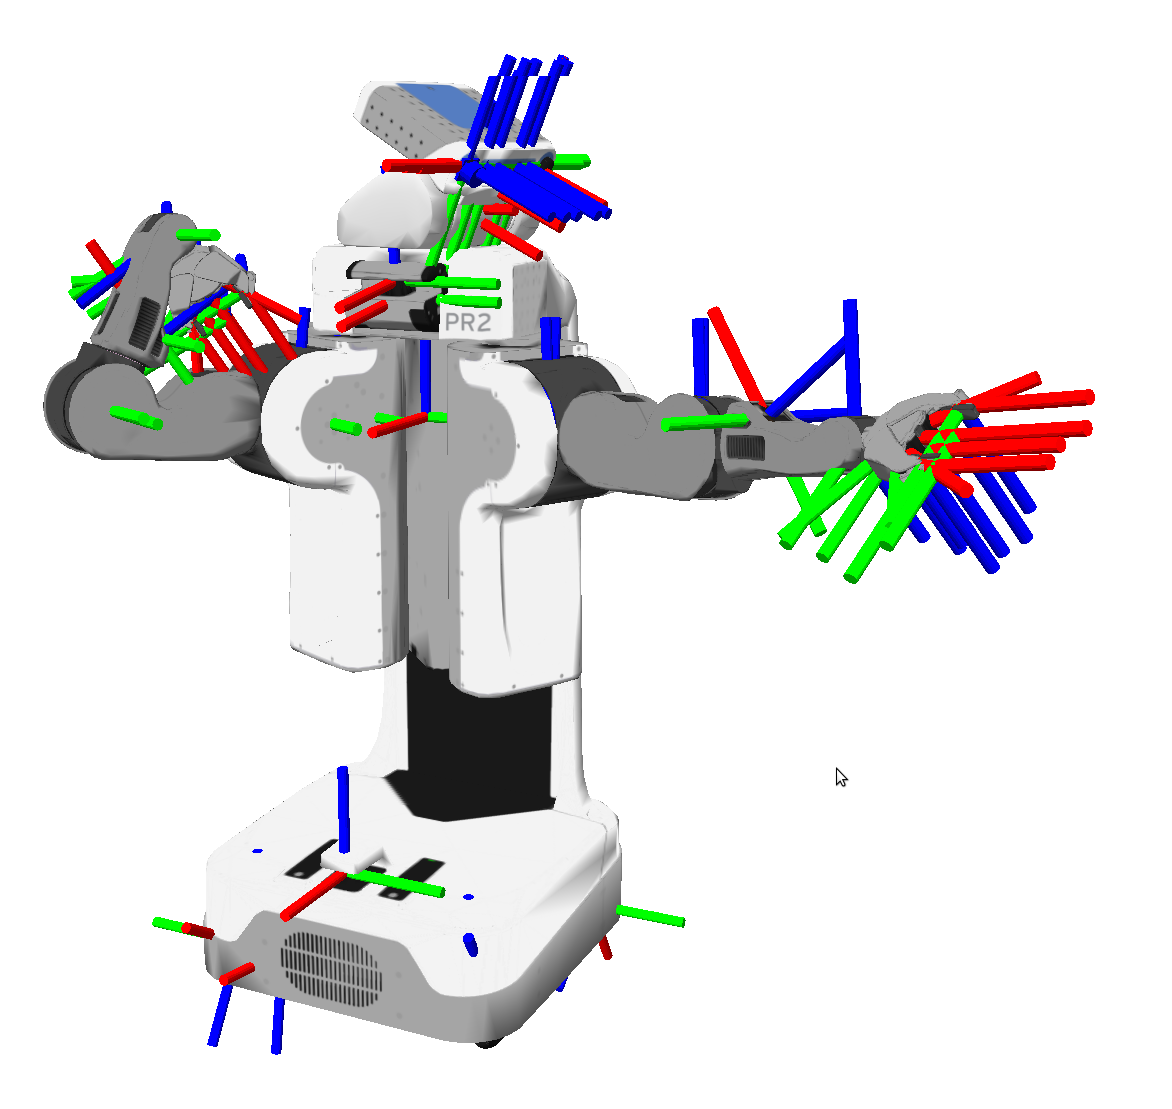
\includegraphics[scale=0.2]{Pictures/robot_multiple_coordinatesystems.png}\\
\end{center}
\caption{Een robot met meerdere coordinate frames met verschillende referentiekaders. De groene, blauwe en rode cilinders  geven de oriëntatie en locaties van de (nulpunten) van de verschillende coordinate frames aan. \tiny{bron: https://wiki.ros.org/tf2}}
\label{fig:coordinateframes}
\end{figure}

\subsection{Broadcasters en TransformStamped messages}
Tf2 helpt ons bij het communiceren van over welke frames we hebben en wat de relatie is tussen de verschillende frames. Dit doen we door middel van \textit{TransformStamped messages}, \textit{broadcasters} en \textit{listeners}. De TransformStamped messages bevatten de informatie over de frames. Een broadcaster publisheert de TransformStamped messages en een listener geeft ons vervolgens de mogelijkheid om de locatie van elke frame te krijgen in het coordinaten stelsel van een andere frame. De listener leggen we uit in sectie \ref{sec:listeners}.

Er zijn twee verschillende broadcasters: gewone \textit{broadcasters} en \textit{static broadcasters}. De static broadcaster geeft performance voordelen als we deze gebruiken voor frames die weinig of nooit veranderen. In codevoorbeeld \ref{code:frameBroadcaster.hpp} zien we de header file van een ROS node class die twee broadcasters heeft als members. 

\begin{lstlisting}[language=C++, caption={frameBroadcaster.hpp; Een node met twee broadcasters. De twee frames maken samen een 1 DOF-robotarm (zie figuur \ref{fig:1DOFRobotarm} en source file in codevoorbeeld \ref{code:frameBroadcaster.cpp}.}, firstnumber=0, label={code:frameBroadcaster.hpp}]
#ifndef _FRAMEBROADCASTER_H_
#define _FRAMEBROADCASTER_H_

#include "rclcpp/rclcpp.hpp"
#include <tf2_ros/transform_broadcaster.h>
#include <tf2_ros/static_transform_broadcaster.h>

class MinimalTF2Broadcaster : public rclcpp::Node
{
public:
  MinimalTF2Broadcaster();
  
private:
    void createArmFrame();
 
    void moveBase();

    rclcpp::TimerBase::SharedPtr timer_;

    tf2_ros::TransformBroadcaster br;
    tf2_ros::StaticTransformBroadcaster sbr;

    double baseAngle_;
};

#endif

\end{lstlisting}

\noindent Voordat de broadcasters een frame kunnen versturen moet dit in een TransformStamped messages worden gestopt. Een TransformStamped message van een frame heeft de volgende velden:
\begin{itemize}
    \item \textbf{header.stamp:} bevat het tijdstip dat de nieuwe frame waar is. Kan worden gebruikt om terug te kijken in de tijd.
    \item \textbf{header.frame\_id:} ook wel parent frame genoemd. We beschrijven in deze message de locatie en orientatie van de frame in de parent frame.
    \item \textbf{child\_frame\_id:} De naam van deze frame.
    \item \textbf{transform.translation.x:} x-coördinaat van het nulpunt van deze frame in de parent frame.
    \item \textbf{transform.translation.y:} y-coördinaat van het nulpunt van deze frame in de parent frame.
    \item \textbf{transform.translation.z:} z-coördinaat van het nulpunt van deze frame in de parent frame.
    \item\textbf{ transform.rotation.x:} x-Quaternion\footnote{Quaternions zijn een manier om de orientatie in een 3D ruimte te beschrijven. Quaternion zijn fijner in gebruik in computerprogramma's. Zie voor meer informatie: \url{https://nl.wikipedia.org/wiki/Quaternion}} van het nulpunt van deze frame ten opzichte van de parent frame.
    \item \textbf{transform.rotation.y:} y-Quaternion van het nulpunt van deze frame ten opzichte van de parent frame.
    \item \textbf{transform.rotation.z:} z-Quaternion van het nulpunt van deze frame ten opzichte van de parent frame.
    \item \textbf{transform.rotation.w:} w-Quaternion van het nulpunt van deze frame ten opzichte van de parent frame.
\end{itemize}
\noindent In codevoorbeeld \ref{code:frameBroadcaster.cpp} zien we de bijbehorende source file van de header file van codevoorbeeld \ref{code:frameBroadcaster.hpp}. In deze source file wordt er een TransformStamped message gemaakt in de functie \textit{createArmFrame()} en in functie \textit{MoveBase()}. De twee frames beschrijven samen een 1 DOF robotarm (zie figuur. \ref{fig:1DOFRobotarm}). De base frame heeft een locatie en oriëntatie in de world frame. De arm frame heeft een locatie en oriëntatie in de base frame. Indirect heeft hiermee de arm frame ook een locatie en orientatie in de world frame. De functie MoveBase() laat de base frame ronddraaien (als een continuous servo). het ronddraaien van de base zorgt er voor dat de arm frame op een andere locatie is in de world frame. De locatie van de arm frame in de base frame blijft echter hetzelfde!

\begin{figure}[ht]
\begin{center}
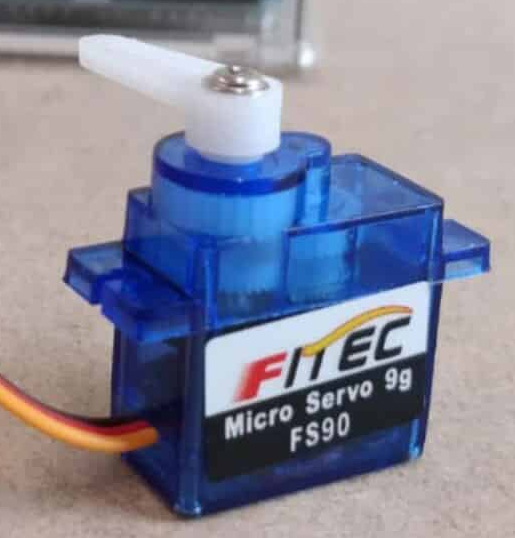
\includegraphics[scale=0.3]{Pictures/1DOFRobotarm.png}\\
\end{center}
\caption{De 1 DOF robotarm. Codevoorbeeld \ref{code:frameBroadcaster.cpp} maakt een frame genaamd 'base' op de locatie van de schroef. Deze kan dus ronddraaien relatief tot de wereld. De frame 'arm' uit codevoorbeeld \ref{code:frameBroadcaster.cpp} zit aan het uiteinde van het witte armpje dat vast zit aan de 'base'.}
\label{fig:1DOFRobotarm}
\end{figure}

\begin{lstlisting}[language=C++, caption={frameBroadcaster.hpp; Een node met twee broadcasters. De twee frames maken samen een 1 DOF-robotarm (zie figuur \ref{fig:1DOFRobotarm}). De base frame definieert zichzelf met een locatie en oriëntatie in relatie tot de world frame. De arm frame doet dit ook, maar dan in relatie tot de base frame.}, firstnumber=0, label={code:frameBroadcaster.cpp}]
#include "frameBroadcaster.hpp"

#include <chrono>

#include "rclcpp/rclcpp.hpp"
#include <tf2_ros/transform_broadcaster.h>
#include <tf2_ros/static_transform_broadcaster.h>
#include <geometry_msgs/msg/transform_stamped.h>
#include <tf2/LinearMath/Quaternion.h>

using namespace std::chrono_literals;

MinimalTF2Broadcaster::MinimalTF2Broadcaster()
  : Node("MinimalTF2Broadcaster"), br(this), sbr(this), baseAngle_(0)
{
    timer_ = this->create_wall_timer(
    500ms, std::bind(&MinimalTF2Broadcaster::moveBase, this));

    createArmFrame()
}

void MinimalTF2Broadcaster::createArmFrame(){:
    geometry_msgs::msg::TransformStamped static_transformStamped;

    static_transformStamped.header.stamp = this->now();
    static_transformStamped.header.frame_id = "base";
    static_transformStamped.child_frame_id = "arm";
    
    static_transformStamped.transform.translation.x = 0;
    static_transformStamped.transform.translation.y = 5;
    static_transformStamped.transform.translation.z = 0.0;

    tf2::Quaternion q;
    q.setRPY(0, 0, 0); // it is easier for humans to think in roll, pitch and yaw.
    static_transformStamped.transform.rotation.x = q.x();
    static_transformStamped.transform.rotation.y = q.y();
    static_transformStamped.transform.rotation.z = q.z();
    static_transformStamped.transform.rotation.w = q.w();

    sbr.sendTransform(static_transformStamped);
}

void MinimalTF2Broadcaster::moveBase()
{
    // change the rotation of the base:
    baseAngle_ += 0.1;

    geometry_msgs::msg::TransformStamped transformStamped;

    transformStamped.header.stamp = this->now();
    transformStamped.header.frame_id = "world";
    transformStamped.child_frame_id = "base";

    transformStamped.transform.translation.x = 5;
    transformStamped.transform.translation.y = 2;
    transformStamped.transform.translation.z = 0.0;

    tf2::Quaternion q;
    q.setRPY(0, 0, baseAngle_); // it is easier for humans to think in roll, pitch and yaw.
    transformStamped.transform.rotation.x = q.x();
    transformStamped.transform.rotation.y = q.y();
    transformStamped.transform.rotation.z = q.z();
    transformStamped.transform.rotation.w = q.w();

    br.sendTransform(transformStamped);
}

\end{lstlisting}

\subsubsection{Broadcasters testen}
\label{sec:broadcastersTesten}
Als we \'e\'en of meerdere frames hebben aangemaakt kunnen we deze testen met Rviz of met tf2\_echo. Met Rviz kunnen we de locaties, orientaties en relaties van de frames visualiseren. Het gebruik van Rviz kan men vinden in de ROS2 documentatie. We laten hier de de simpelere test met Tf2\_echo zien. Tf2\_echo geeft ons de locatie en oriëntatie van een frame in het stelsel van een andere frame. Om codevoorbeelden \ref{code:frameBroadcaster.hpp} en \ref{code:frameBroadcaster.cpp} te testen kunnen we kijken waar de arm frame zich bevind in de world frame. We doen dat door de node te runnen en in de een andere terminal het volgende uit te voeren\footnote{Het complete voorbeeld in een werkende package is te vinden in de .zip met voorbeelden.}:

\begin{lstlisting}[style=DOS, caption={}, firstnumber=0, label={}]
ros2 run tf2_ros tf2_echo world arm
\end{lstlisting}

\noindent Als de code goed werkt zien we dat de locatie van de arm steeds veranderd\footnote{De x-coördinaat loopt van 0 tot 10 en de y-coordinaat van -3 tot 7}\footnote{nog even kijken of de code in de voorbeelden niet is geupdate. Ik dacht dat hier iets mee was.}. We kunnen ook testen of inderdaad de arm frame wel gelijk blijft in relatie tot de base frame:

\begin{lstlisting}[style=DOS, caption=Hello world, firstnumber=0, label={}]
ros2 run tf2_ros tf2_echo base arm
\end{lstlisting}

\noindent Maar we kunnen de zaken ook van de andere kant bekijken. Soms wil juist vanuit het component redeneren in plaats vanuit de wereld. Je kan dus ook vragen waar het nulpunt van de world is in het coördinaten stelsel van de arm frame:

\begin{lstlisting}[style=DOS, caption=Hello world, firstnumber=0, label={}]
ros2 run tf2_ros tf2_echo arm world
\end{lstlisting}


\subsection{Listeners}\label{sec:listeners}
In sectie \ref{sec:broadcastersTesten} zien we hoe we met een command in de terminal de locatie en oriëntatie van een frame in een andere frame kunnen zien. Dit willen we natuurlijk ook in onze code kunnen doen. Hiervoor gebruiken we de \textit{listeners} van tf2. Listeners krijgen transformStamped messages binnen waarin de locatie en oriëntatie zit van een frame in het stelsel van een andere frame. In codevoorbeeld \ref{code:frameListener.hpp} zien we een de .hpp van een node class die een listener heeft. Naast de listener heeft de node ook een buffer als member. De listener maakt gebruikt van deze buffer. In codevoorbeeld \ref{code:frameListener.cpp} zien we de source van deze node. In de constructor (en specifiek de initializer lists) zien we het declareren van de buffer en de listener. In \textit{listenAndPrint()} wordt de TransformStamped van de arm frame in relatie tot de world frame opgehaald en geprint op het scherm.

\begin{lstlisting}[language=C++, caption={frameListener.hpp; De header file van een node met een listener.}, firstnumber=0, label={code:frameListener.hpp}]
#ifndef _FRAMElISTENER_H_
#define _FRAMElISTENER_H_

#include "rclcpp/rclcpp.hpp"
#include <tf2_ros/transform_listener.h>
#include <tf2_ros/buffer.h>

class MinimalTF2Listener : public rclcpp::Node
{
public:
    MinimalTF2Listener();

private:

    void listenAndPrint();

    rclcpp::TimerBase::SharedPtr timer_;

    tf2_ros::Buffer tfBuffer;
    tf2_ros::TransformListener tfListener;
};

#endif

\end{lstlisting}


\begin{lstlisting}[language=C++, caption={frameListener.hpp; De header file van een node met een listener.}, firstnumber=0, label={code:frameListener.cpp}]
#include "frameListener.hpp"

#include <chrono>

#include "rclcpp/rclcpp.hpp"
#include <tf2_ros/transform_listener.h>
#include <tf2_ros/buffer.h>
#include <geometry_msgs/msg/transform_stamped.h>
#include <tf2/LinearMath/Quaternion.h>

using namespace std::chrono_literals;

MinimalTF2Listener::MinimalTF2Listener()
    : Node("MinimalTF2Listener"), tfBuffer(this->get_clock()), tfListener(tfBuffer)
{
    timer_ = this->create_wall_timer(
        500ms, std::bind(&MinimalTF2Listener::listenAndPrint, this));    
}


void MinimalTF2Listener::listenAndPrint()
{
    geometry_msgs::msg::TransformStamped transformStamped;

    
    try{ // try to get the coordinates of arm in the world frame:
        transformStamped = tfBuffer.lookupTransform("world", "arm", tf2::TimePoint());
    }
    // otherwise explain what went wrong and exit this function:
    catch (const tf2::TransformException & ex) {
        std::cout << "Failure at " << this->now().seconds() << std::endl;
        std::cout << "Exception thrown:" << ex.what() << std::endl;
        std::cout << "The current list of frames is:" << std::endl;
        std::cout << tfBuffer.allFramesAsString() << std::endl;
        return;
    }

    RCLCPP_INFO(this->get_logger(), "The arm is at: (%.5f,%.5f,%.5f)", 
                    transformStamped.transform.translation.x,
                    transformStamped.transform.translation.y,
                    transformStamped.transform.translation.z);
}



\end{lstlisting}

\subsection{Meer informatie:}
De tutorials van tf2 met ROS 2 zijn nog erg minimalistics\footnote{\url{https://index.ros.org/doc/ros2/Tutorials/tf2/}}. Gelukkig is de werking van tf2 niet verandert met de overgang van ROS 1 naar ROS 2. De ROS 1 informatie van tf2 is ook voor ROS2 een goede bron. Let wel op: ROS 1 heeft een andere manier van het maken en opstarten van nodes. Op de onderstaande link vind je meer informatie over tf2:

\begin{center}
    \url{https://wiki.ros.org/tf2}
\end{center}


\section{Rviz} \label{sec:rviz}
In de voorbeelden .zip is een werkend voorbeeld met Rviz te vinden.